\documentclass[twocolumn]{aastex631}
\usepackage{graphicx}
\usepackage{physics}
\usepackage[super]{nth}
\usepackage{enumitem}

\begin{document}
\title{Using Hybrid Machine Learning for Fundamental Stellar Parameter Inference}
\author[0000-0002-2290-6810]{Sujay Shankar}
\author[0000-0002-4020-3457]{Michael Gully-Santiago}
\author[0000-0002-4404-0456]{Caroline V. Morley}
\affil{Department of Astronomy, The University of Texas at Austin, Austin, TX 78712, USA}

\begin{abstract}
    Text
\end{abstract}
\keywords{Text}

\section{Introduction}
Stellar spectra are exceedingly rich sources of information about the stars
which create them. They contain information about the fundamental properties
of the star such as its temperature and surface gravity, as well as
countless absorption lines reflecting the star's chemical composition. On 
top of that, extrinsic factors such as the radial velocity of the star or 
the rotation of the star itself further transform spectra. When these spectra
are observed, even the location of the observing instrument and the 
capabilities of the instrument itself introduce further modifications. 
In short, stellar spectra represent extremely complex, high-dimensional 
data that has gone through multiple transformations before reaching our 
eyes as a deceptively simple graph of flux versus wavelength.

Scientists want to extract as much information as possible from
a star's spectra to get back the properties that lie at the root of it all. 
However, this has proven to be no easy task. Spectroscopic surveys such as 
APOGEE develop their own in-house pipelines to extract stellar parameters
from spectra (ASPCAP in the case of APOGEE), and these pipelines are fairly
effective. However, they all work on the core assumption that the data to be 
analyzed is a list of pixels. In addition, the pipelines that surveys 
develop are typically closed-source and usually limited to the scope of the 
survey itself, causing a sort of fragmentation. This motivates the 
development of a more universal, open-source tool that can do what spectral 
analysis pipelines do, but in an alternative way. 

Multiple efforts have been made in this direction, treating spectra in 
different ways. The standard practice is to treat the wavelength and flux as 
simply two arrays and implement any from a myriad of different algorithms to 
inference fundamental stellar parameters. Others take a more mathematical 
approach by decomposing spectra into some eigenbasis and treating it as a 
regression problem, such as \texttt{starfish}. However, \texttt{blase} takes 
a different approach. It treats spectra not as a set of pixels or a set of 
eigenbasis coefficients but as a set of spectral lines, specifically Voigt 
profiles. There is no metric of this approach being better or worse than the 
others mentioned so far, but it is a different paradigm and is worth 
exploring as a semi-empirical tool. This study aims to take advantage of 
\texttt{blase}'s ability to change a spectrum's basis from flux versus 
wavelength into spectral line versus spectral line properties, and use that 
to develop a robust tool for stellar parameter inference.

However, this is only a proof of concept. Here we develop a tool that 
represents a very basic realization of the idea of line-by-line inference. 
We make no claims as to the performance of this tool, but rather aim to show 
that the idea is sound and able to be implemented, even if rudimentary, and 
that with further research and development, this tool has the potential to 
become useful for spectral inference.

We chose the PHOENIX synthetic spectral model grid as the basis for this 
study, because it is fairly well-known. While we plan to extend this tool to 
leverage information across multiple model grids in the future, both for 
accuracy and to increase the scope to include substellar objects with grids
such as Sonora, for now we limit our scope to a subset of the PHOENIX grid.

\section{Cloning the PHOENIX Model Grid}
\subsection{The PHOENIX Subset}
For the purposes of this study, we did not consider the full range of the
PHOENIX synthetic spectral model grid. Instead, we focused on a subset of 
the grid, whose parameter ranges are given in Table 1.

\begin{table}[h!]
    \hspace*{-1.35cm}\begin{tabular}{|c|c|c|}
        \hline
        \multicolumn{3}{|c|}{\textbf{PHOENIX Grid Subset}}\\
        \hline\hline
        Parameter & Symbol & Range\\
        \hline
        Alpha Element Abundance & $\alpha$ & [0] dex\\
        Iron Abundance & [Fe/H] & [-0.5, 0] dex\\
        Effective Temperature & $T_{\mathrm{eff}}$ & [2300, 12000] K\\
        Surface Gravity & $\log(g)$ & [2, 6]\\
        Wavelength & $\lambda$ & [8038, 12849] \AA\\
        \hline
    \end{tabular}
    \caption{The subset of the PHOENIX grid used in this study. These limits 
    were imposed to reduce the computational cost of the algorithms and to 
    ensure a rectilinear parameter space in order to work with \texttt{scipy}'s
    \texttt{RegularGridInterpolator}. The wavelength limits in particular 
    roughly line up with that of the Habitable Zone Planet Finder (HPF) 
    spectrograph. This subset is comprised of 1314 individual spectra.}
\end{table}

\subsection{Preprocessing with \texttt{gollum}}
First, the PHOENIX subset was accessed directly from the PHOENIX website
using \texttt{gollum}'s download option. The spectra were then put through a 
three-step preprocessing pipeline.
\begin{enumerate}
    \item \textit{Blackbody Division}: Since the $T_{\mathrm{eff}}$ of each spectrum 
    is known, the according blackbody spectrum was divided out.
    \item \textit{Percentile Normalization}: The spectra were normalized by dividing
    them by their 99th percentile.
    \item \textit{Continuum Normalization}: The spectra were further normalized by 
    dividing them by a \nth{5} order polynomial continuum.
\end{enumerate}
Mathematically, we can express the preprocessing as follows:
\begin{gather}
    \mathsf{\bar{S}} = \dfrac{\mathsf{S}}{\mathsf{B}\mathsf{Q}_5P_{99}}
\end{gather}
where $\mathsf{\bar{S}}$ is the preprocessed spectrum, $\mathsf{S}$ is the 
original spectrum,  $\mathsf{B}$ is the blackbody spectrum, $\mathsf{Q}_n$ 
is the $n^\mathrm{th}$ order polynomial continuum fit, and $P_n$ is the 
$n^\mathrm{th}$ percentile function. Arithmetic operations between arrays 
are assumed to be elementwise in all notation from here on out.

\subsection{Line Identification with \texttt{blase}}
The next step was to convert the PHOENIX subset into an interpretable format.
We wanted to represent the spectra as a list of spectral lines rather than a
list of fluxes. This was done using \texttt{blase}, which detects spectral 
lines as Voigt profiles and tunes the profiles to mimic the original 
PHOENIX spectrum with back propagation. Four parameters were optimized: the 
line center $\mu$, the log-amplitude $\ln(a)$, the Gaussian width $\sigma$, and the 
Lorentzian width $\gamma$. The optimization used the Adam optimizer with a
learning rate of 0.05 over 100 epochs. In addition, we limited two custom 
parameters: wing cut to 6000 and prominence to 0.005. Wing cut is a parameter
that determines the extent of the Voigt profile to evaluate, saving
computational resources by not evaluating small numbers. Prominence sets a
lower limit for the amplitude of detected lines, which also saves resources 
by disregarding shallow lines. In short, larger values for wing cut and 
smaller values for prominence both increase the accuracy of using
\texttt{blase}'s line detection and optimization at the expense of an
increased computational cost.

Once optimization was complete, the list of identified lines, present in the
state dictionary of \texttt{blase}'s model, was saved to a \texttt{.pt} file
for each PHOENIX subset grid point. The total disk space these files took up 
is 465 MB.

\section{Interpolating Manifolds}
\subsection{Cross-Model Line Identification}
Earlier we mentioned that \texttt{blase} tuned the line centers of
detected lines. This means that from one PHOENIX spectrum to the next, the
same line could have a slightly different line center. Since the goal of this
study is to interpolate the properties of each line, we needed to identify the
presence of a particular line across the PHOENIX subset. We decided to do
this by using the line centers $\mu$ of the detected lines pre-optimization, 
while the post-optimization line centers are labeled $\mu'$. Now with 
each spectral line indexed by $\mu$, we had four parameters to interpolate:
$\mu'$, $\ln(a)$, $\sigma$, and $\gamma$. Mathematically, the Voigt profile
$\mathsf{V}_\mu$ in terms of our four parameters is given by:

\begin{gather}
    \mathsf{V}_\mu(\lambda) = e^{\ln(a)}\mathrm{Re}\left[w\left(\dfrac{\lambda - \mu' + i\gamma}{\sigma\sqrt{2}}\right)\right] \bigg/ \left(\sigma\sqrt{2\pi}\right)
\end{gather}
where $w$ is the Faddeeva function. Note that since we are dealing with 
the parameters of these Voigt profiles, even if the interpolation method is 
linear, the actual result of interpolation varies non-linearly.

There is also a second issue, and that is that spectral lines were often
only detected in some spectra from the PHOENIX subset. In Figure 1, we show
that different grid points sport differing counts of detected spectral lines.
This means that in theory, interpolation would be inaccurate in regions where 
a line does not appear, and also breaks in practice because \texttt{scipy}'s 
\texttt{RegularGridInterpolator} relies on a rectilinear grid, which we would not 
have if regions of grid points were missing. 

\begin{figure*}[t!]
    \centering
    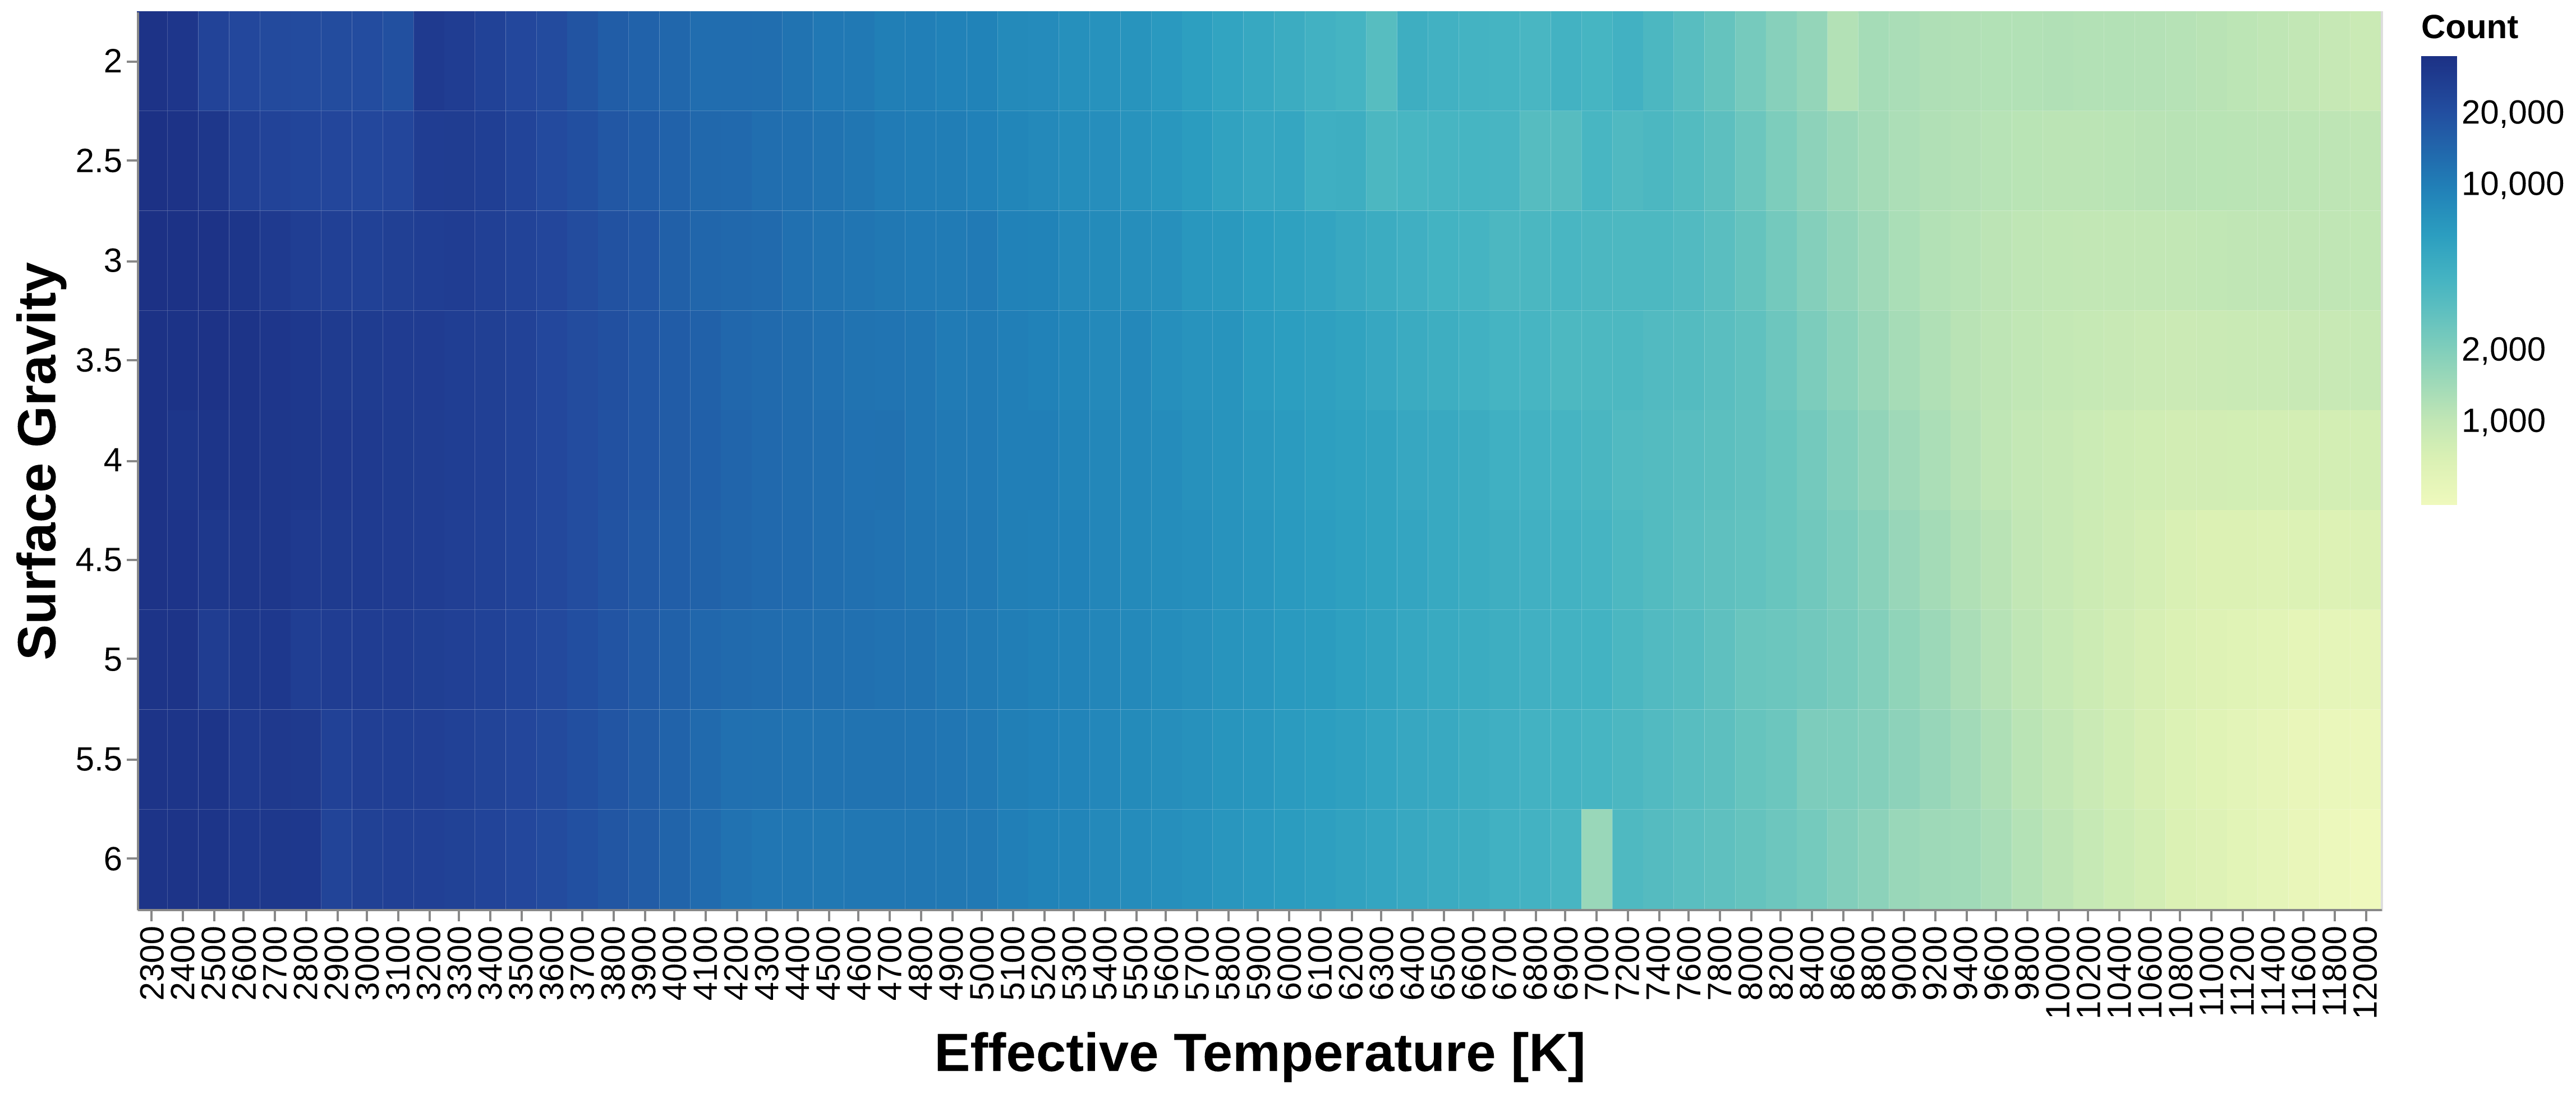
\includegraphics[width=\textwidth]{images/figure1.png}
    \caption{The number of detected spectral lines at each grid point of 
    a slice of the PHOENIX subset at solar metallicity. We can see that
    the number of detected lines decreases with increasing $T_{\mathrm{eff}}$.
    Also note that from $T_{\mathrm{eff}} = 7000$ K onward, the spacing 
    between grid points increases from 100 K to 200 K.}
\end{figure*}

To solve this, we artificially
populated missing grid points with log-amplitudes of -1000, which retained
interpolator stability by not being an infinity, but also essentially 
nullified the line when evaluated. An example of the appearance of missing 
sections in heatmaps where a line does not appear is shown in Figure 2. 
In total, across the entire PHOENIX subset, \texttt{blase} detected 
128,723 individual spectral lines, meaning we have that many manifolds to 
interpolate.

\begin{figure*}[t!]
    \centering
    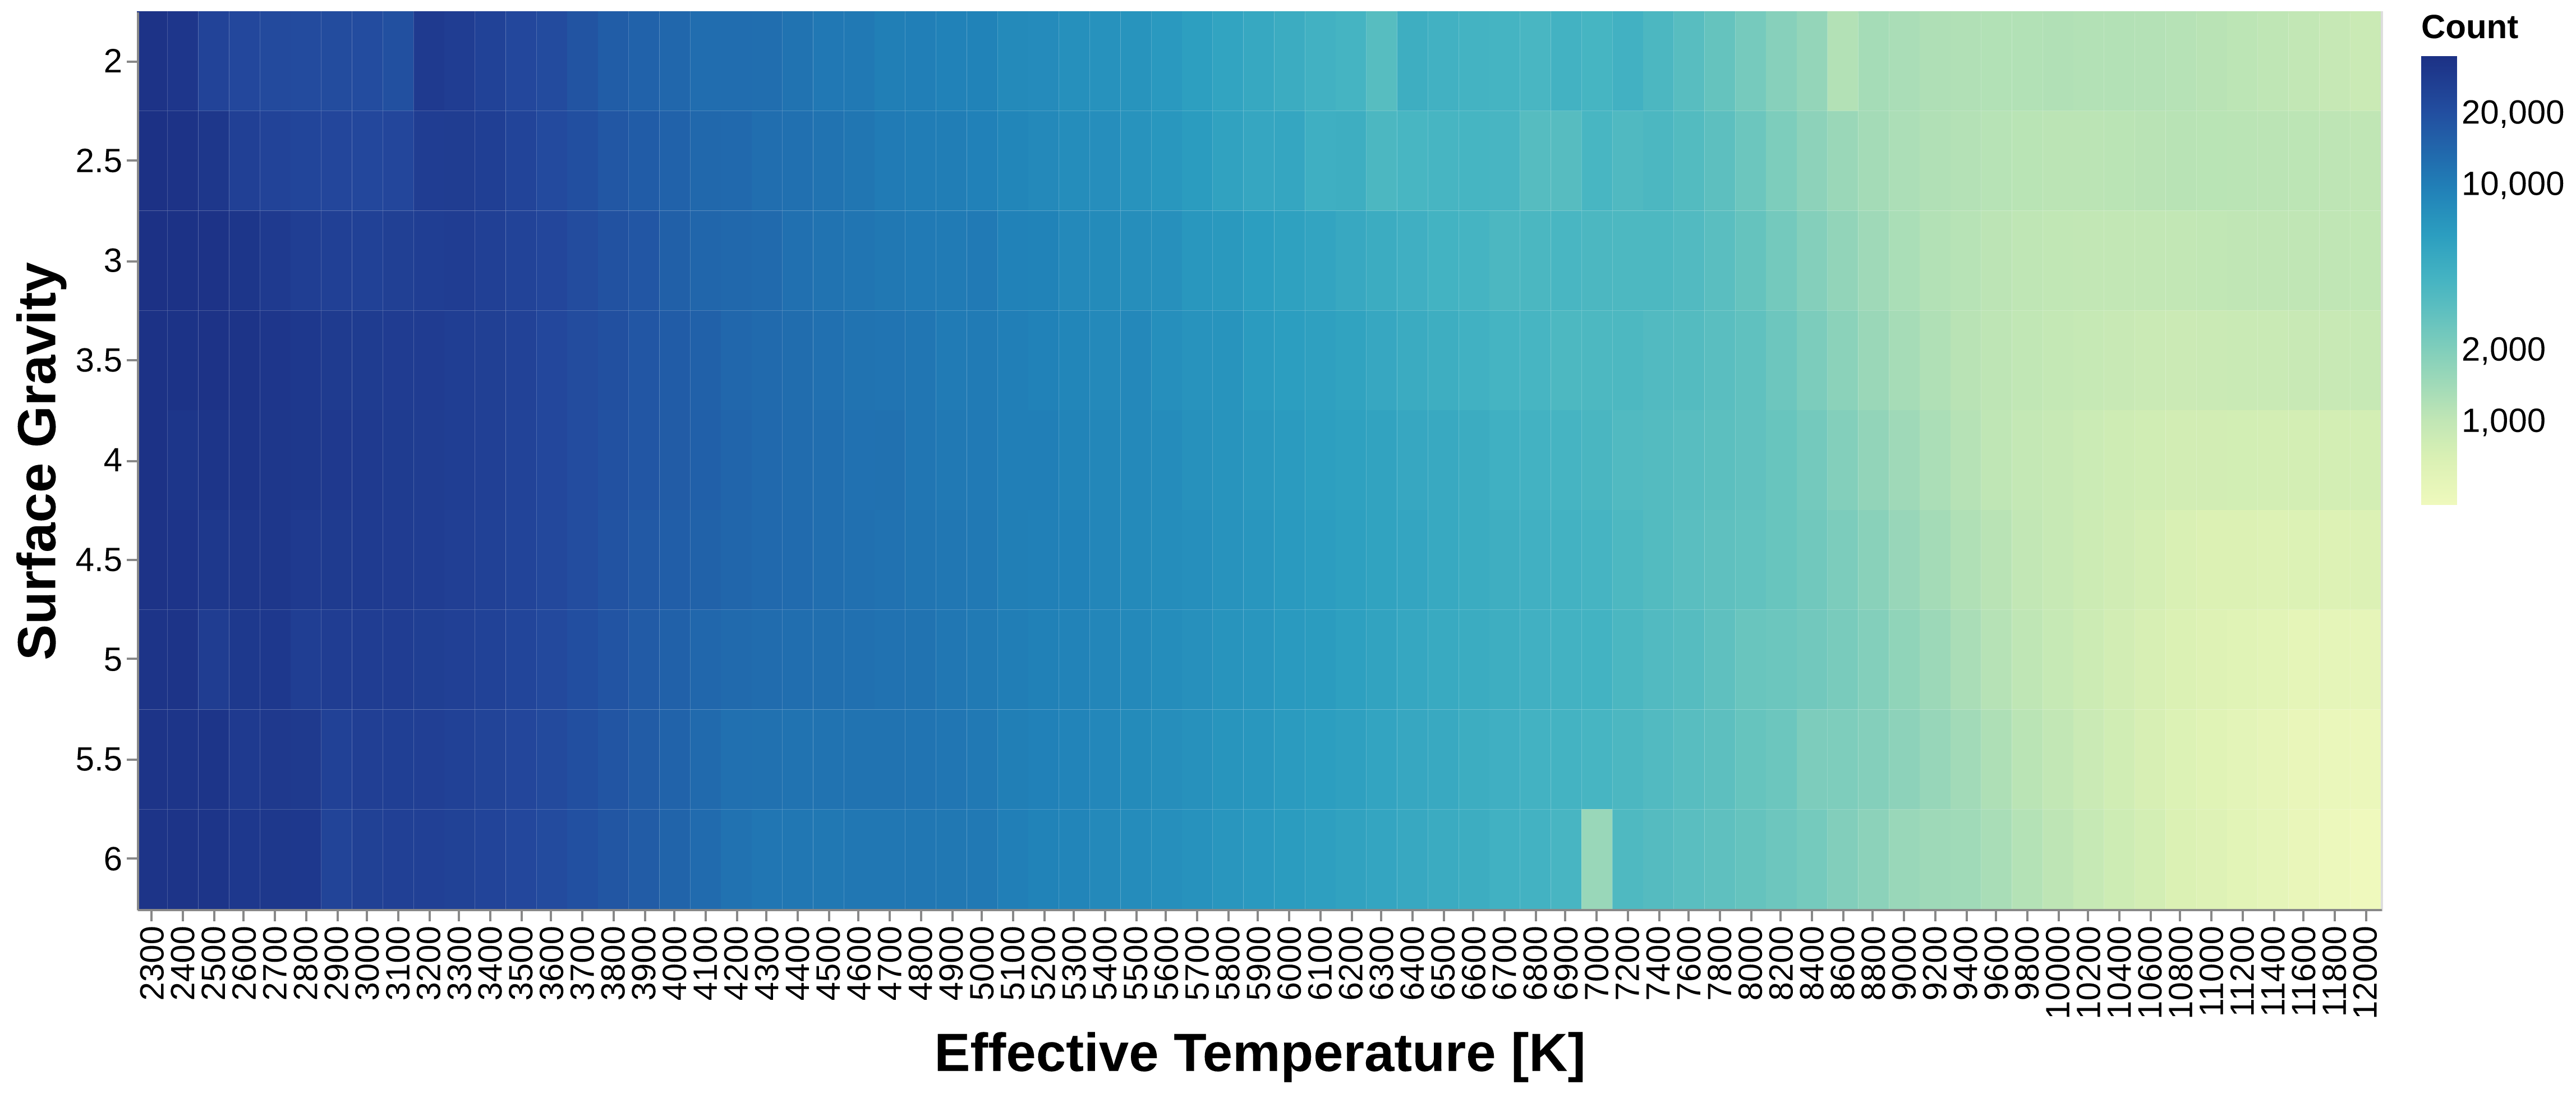
\includegraphics[width=\textwidth]{images/figure2.png}
    \caption{Heatmap showing how $\ln(a)$ varies over the PHOENIX subset
    slice at solar metallicity. Notice the missing chunk in the top left
    of the figure; \texttt{blase} did not detect a spectral line here,
    but we have to artificially populate those points with lines that 
    have $\ln(a) = -1000$.}
\end{figure*}

\subsection{Continuously Evaluable Manifolds}
For each line, the inputs to the interpolator were the three input parameters $T_{\mathrm{eff}}$,
$\log(g)$, and [Fe/H], and the output was a list of four parameters, 
$\mu'$, $\ln(a)$, $\sigma$, and $\gamma$. For each line, one of these 
interpolator objects was created using linear interpolation, and these 
interpolators were aggregated into a single list, which was when pickled 
and written to a \texttt{.pkl} file. These interpolators generate multiple 
manifolds with the following mapping:
\begin{gather}
    \mqty[T_{\mathrm{eff}} \\ \log(g) \\ \mathrm{[Fe/H]}] \rightarrow \mqty[\mu' \\ \ln(a) \\ \sigma \\ \gamma]
\end{gather}
These interpolators could now be evaluated at any point lying within the 
domain of the PHOENIX subset, turning a discretely sampled PHOENIX subset 
into a continuous one. With the given size of the PHOENIX subset, the 
interpolator list takes up 13.2 GB of disk space. Since this is now evaluable,
we call this the PHOENIX generator.

\section{Bayesian Inference and Testing}
\subsection{Inference Algorithm}
With the PHOENIX generator complete, we used Bayesian optimization as the
inference algorithm, specifically the \texttt{gp\_minimize} function from
the \texttt{scikit-optimize} library. This algorithm uses a Gaussian Process
to model the objective function, which in this case was the RMS 
(Root-Mean-Square) loss between the interpolated spectrum and the true 
spectrum. The optimizer was configured to first run 30 random evaluations to 
seed the surrogate model, then run 20 more evaluations now guided by the 
surrogate model. This totals to 50 evaluations, which was deemed sufficient 
for this study. We then decided to use ensemble methods, running 32 parallel
optimizers to get a more statistically sound result. One inference run 
takes an average of 15 minutes to complete on Triton (see Section 5 for
specifications).

\subsection{Test Data}
To test the performance of the inference algorithm, we used the PHOENIX subset
itself. At first glance, this may seem like a useless endeavor, as the 
PHOENIX generator has indeed memorized the PHOENIX subset, being able to
reconstruct a PHOENIX spectrum when evaluated at that grid point. However,
that is precisely what allows us to use the PHOENIX subset as test data.
The Bayesian optimizer's surrogate model is seeded by random continuously 
sampled generator evaluations within the search space, \textit{not} grid 
points of the PHOENIX subset, meaning the surrogate model has no `memorization' 
to speak of. If the optimizer had been an iterative grid refinement search, 
this would not have been possible, because grid methods rely on just that, 
the grid.

\subsection{Performance Results}
Text

\section{Discussion}
The computer used for this study, Triton, has the following specifications:
\begin{table}[h!]
    \hspace*{0.6cm}\begin{tabular}{|c|c|}
        \hline
        \multicolumn{2}{|c|}{\textbf{Triton Specs}}\\
        \hline\hline
        CPU & AMD EPYC 7513\\
        Memory & 256 GB\\
        GPU & Nvidia A100 40GB ($\times$2)\\
        \hline
    \end{tabular}
    \caption{This computer is owned by Caroline Morley and is available to
    members of her research group. It was used for all computations, but not 
    for generating visualizations. The EPYC 7513 is a 32c/64t CPU with a 
    boost clock of 3.65 GHz.}
\end{table}

It should be noted that this study represents a proof of concept, and that 
there are numerous design considerations that could be improved upon with 
future work. These considerations include but are not limited to the 
following:
\begin{enumerate}[label=-]
    \item \textit{Limited PHOENIX Subset}: The PHOENIX subset used in this 
    study was just that, a subset. The full PHOENIX grid not only expands 
    the [Fe/H] range to [-4.0, 1.0] dex and the $\log(g)$ range to [0, 6], 
    but also includes the alpha element abundance parameter, which we 
    elected to fix at 0 for this study. In addition to the actual fundamental 
    stellar parameters, we also took a subset of the PHOENIX wavelength range, 
    with the full [500, 55000] \AA \ wavelength range also being left to 
    future work.
    \item \textit{Strict Wavelength Range}: Currently, the generator only 
    supports inference on spectra whose wavelength limits are either equal 
    to it, or encompass that of the generator and have been truncated to 
    match. However, when the spectrum in question has a smaller wavelength 
    range than the generator, currently there is no functionality to truncate 
    the generator. This would require externally indexing the generator's 
    individual interpolators by line center position and selectively
    evaluating those to eliminate wasteful computation.
    \item \textit{Low-Order Interpolation}: The current design of the 
    algorithm uses linear interpolation to construct manifolds, however this
    could be made more sophisticated with more complex interpolation schemes.
    However, the drawback of this is that higher orders of interpolation
    become increasingly expensive both in terms of disk utilization, and 
    in terms of the computational cost to generate and evaluate them. Future
    studies should sidestep this issue by using more generalizable methods
    that are much more efficient.
    \item \textit{Single Model Grid}: The PHOENIX grid is not the only model
    grid of synthetic spectra available, and it does not apply to all types 
    of stars. Future work would extend the reach of this study's algorithm 
    to encompass other model grids such as the Sonora series for substellar
    models. \texttt{blase} should be able to have an option for the user to 
    input which model grid they would like to base the inference on, and 
    to get even more advanced, perhaps even have the ability to intelligently
    determine which model grid to use automatically.
    \item \textit{Memorization vs.\ Generalization}: The current design of
    the algorithm constructs manifolds using interpolation. This means that
    performance is good at points close to PHOENIX subset grid points, but
    is highly dependent on the type of interpolation used. As interpolators
    require memorization of the data, advanced interpolation becomes extremely
    expensive in terms of disk utilization. Future work would involve 
    constructing manifolds using regression, which would allow for much
    better generalization and lower disk utilization at the expense of
    some accuracy.
    \item \textit{Extrinsic Absence}: The current design of our algorithm
    does not account for extrinsic parameters that modify the appearance of 
    spectra such as rotational broadening and doppler shifting. Future work
    would need to develop ways to tune these extrinsic parameters alongside
    the fundamental stellar parameters.
    \item \textit{Framework Overhead}: As this algorithm is currently more 
    proof of concept than practical, it uses convenience functions from 
    various libraries, which naturally introduces some level of overhead and 
    leaves performance on the table. Future work would involve writing 
    custom functions expressly designed for \texttt{blase}, most likely a 
    complete rewrite of the library from the ground up.
    \item \textit{Pseudo-Interpretability}: Our algorithm boasts interpretability
    by considering spectral lines as the objects of interest as opposed to 
    the rather uninterpretable flux values of other approaches. However, this
    is only a step in the direction of interpretability. True interpretability
    would decompose a spectrum not into a set of spectral lines, but into a
    set of species component spectra, which requires a much more advanced 
    understanding of different species and their behavior, as well as
    direct access to a radiative transfer code as opposed to an off-the-shelf
    model grid. This approach would also extend the inference from just
    fundamental stellar parameters defined by a grid to any set of parameters
    accounted for in the radiative transfer model, down to specific species
    abundances.
    \item \textit{The Continuum Black Box}: Continuum normalization is a
    process that is not yet completely understood, and is currently done as 
    a preprocessing step with a fairly simple algorithm. Future work would
    dive deeper into the science of continuums and develop more advanced 
    methods that can discern continuums with greater accuracy and less
    modeling restrictions.
    \item \textit{One Voigt Fits All}: The current assumption of \texttt{blase}
    is that every spectral line is a Voigt profile. This assumption is largely
    true, but there are situations where that is simply not enough. Future
    studies need to account for more advanced spectral line profiles and 
    procedures to deal with phenomena such as ro-vibrational bands.
\end{enumerate}
In short, it is quite clear that \texttt{blase} is a long way from being a
powerhouse in spectral inference, however it represents a step down a road
not yet traveled, and the potential for future growth is immense. At the 
end of the day, we aim to develop a tool that can analyze spectra with the 
advent of physics-informed machine learning.

\section*{Acknowledgements}
Text

\end{document}